\problemname{Godiskross}

I den här uppgiften ska vi spela en mycket förenklad version av ett populärt dataspel som vi kan kalla Godiskross. I vår version är spelplanen en enda stapel med $R$ rutor. I varje ruta finns en godisbit som kan vara av tre olika sorter (låt oss kalla dem A, B och C). I spelet får du göra upp till $M$ drag. I varje drag ska du byta plats på två intill-liggande godisbitar så att en sekvens med minst tre lika godisbitar bildas. Om du inte kan göra något drag är spelet slut.

När du gjort ett drag krossas (försvinner) alla godisbitar som ingår i en sådan sekvens (observera att det kan finnas flera sekvenser och alla försvinner samtidigt). Därefter fylls alla hål igen genom att godisbitar som ligger i rutorna ovanför ramlar ned (se figuren nedan). Det fylls alltid på med nya godisbitar så att spelplanen är full. För att veta vilka nya bitar som ramlar in ovanifrån ska du tänka dig att den ursprungliga stapeln är kopierad uppåt i en oändligt hög stapel (se figuren nedan).

När hålen fyllts igen uppstår en ny situation och processen upprepas automatiskt: alla godisbitar som ingår i sekvenser försvinner och hålen fylls igen. Detta fortsätter tills inga sekvenser längre finns på spelplanen. Då är det dags att göra nästa drag.

Spelets poängräkning är enkel. Varje gång en sekvens med minst tre godisbitar uppstår (genom ditt drag eller genom nedramling) får du $(2L-5)$ poäng där $L$ är sekvensens längd. En sekvens med tre godisbitar ger alltså 1 poäng, en med fyra bitar ger 3 poäng o.s.v.

Skriv ett program som, givet den ursprungliga stapeln och det maximala antalet drag du får göra, beräknar den maximala poängen du kan uppnå.

\begin{figure}[ht!]
\centering
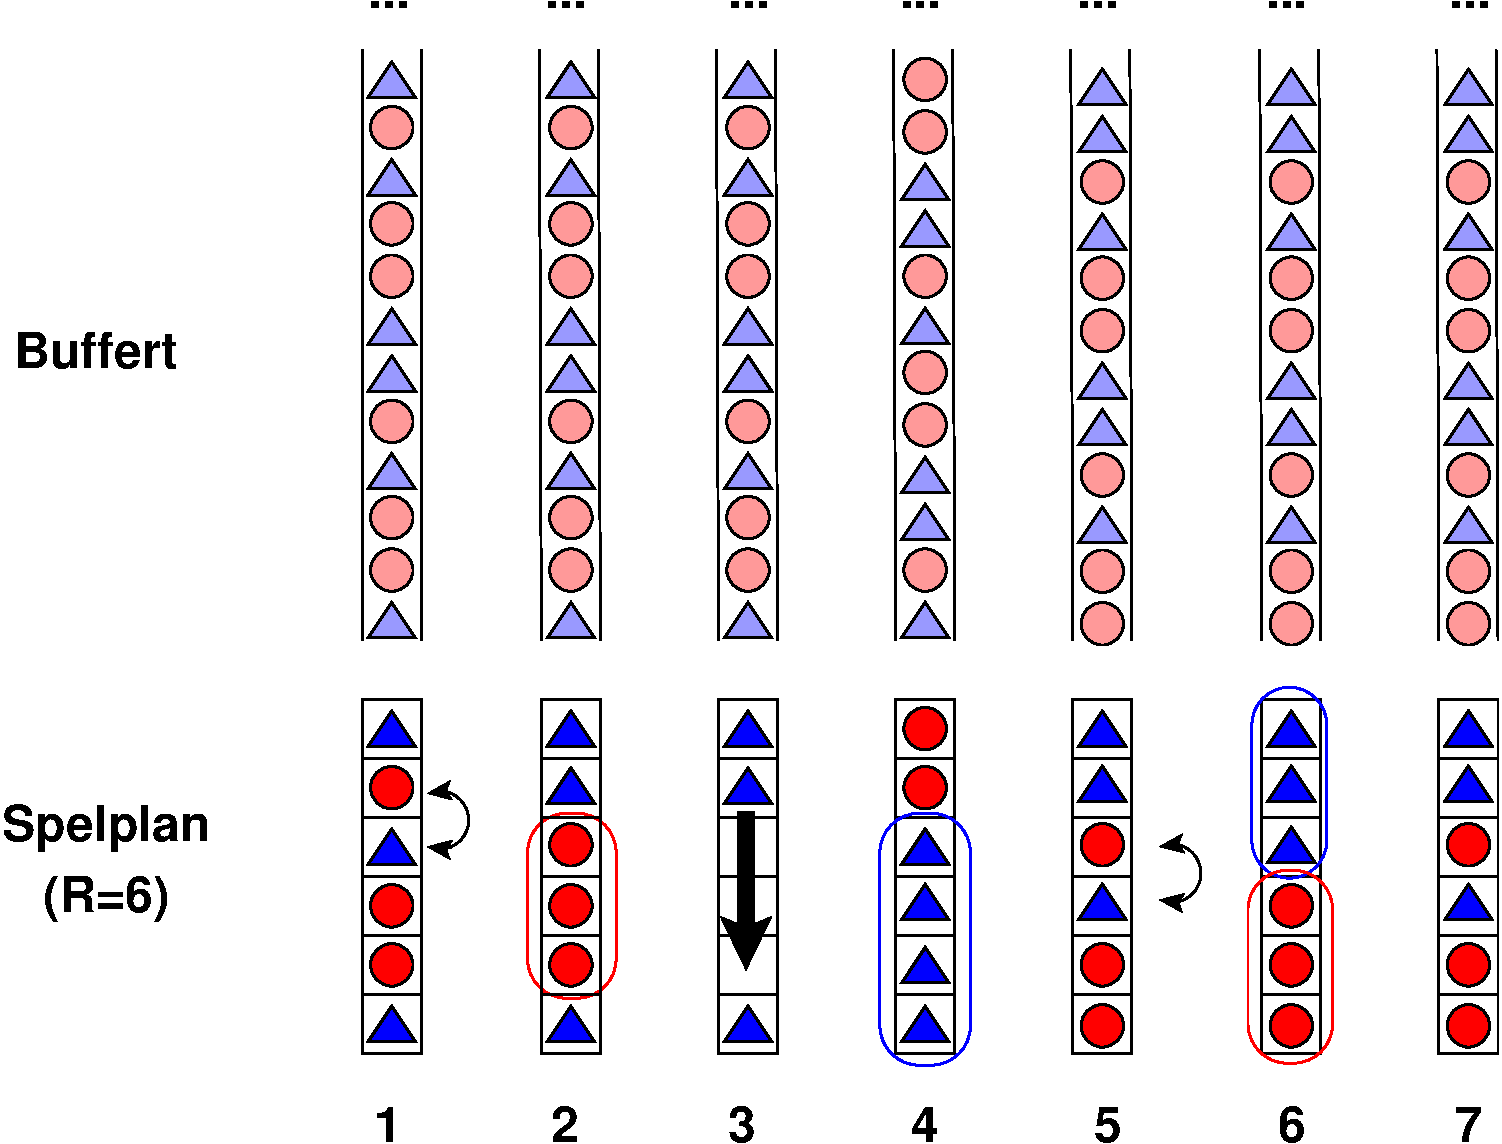
\includegraphics[width=0.7\textwidth]{godiskross_exempel.pdf}
\caption{Händelseförloppet i första exemplet (bild 1--5) och andra exemplet (bild 1--7). I indata kallas röda cirklar A och blåa trianglar B. Den övre delen av figuren symboliserar en tänkt buffert av godis som ramlar ner när godis krossas. I ursprungsställningen (bild 1) kan du endast göra ett drag (markerat med pilar). Då bildas en röd 3-sekvens som ger 1 poäng (bild 2). När godisbitarna krossas bildas ett hål som fylls igen genom att bitar ovanför ramlar ned (bild 3). 
Då uppstår en blå 4-sekvens som ger 3 poäng (bild 4). När dessa bitar krossas uppstår en situation utan sekvenser och första draget är färdigt (bild 5). Om du får göra ytterligare ett drag bildas två sekvenser som ger vardera 1 poäng (bild 6). Observera att du {\em inte} kan låta den blå sekvensen krossas först för att på så sätt få en röd 5-sekvens, utan båda sekvenserna försvinner samtidigt och ger slutställningen (bild 7). Totalpoängen för de två dragen blir $1+3+1+1=6$}
\label{overflow}
\end{figure}

\section*{Input}
På första raden står heltalet $N$, det maximala antalet drag du får göra ($1 \le N \le 5$). På andra raden står en sträng med $R$ bokstäver ($3 \le R \le 20$), valda bland A, B och C. Detta är den ursprungliga stapeln, beskriven nedifrån och upp. Tre lika bokstäver förekommer aldrig i följd. Indatan är vald så att inga oändliga nedramlings-loopar kan uppstå.

\section*{Output}
Programmet ska skriva ut ett heltal -- den maximala poängen du kan uppnå.


\section*{Poängsättning}
Din lösning kommer att testas på en mängd testfallsgrupper. För att få poäng för en grupp
så måste du klara alla testfall i gruppen.

\begin{tabular}{| l | l | l |}
\hline
Grupp & Poängvärde & Gränser \\ \hline
1--3     & 30         & $N=1$ \\ 
4--10     & 70         & $2 \le N \le 5$ \\ \hline
\end{tabular}

